% conclusion
%
% CONCLUSION: Limitations of the study, Questions for further research.
%
%----------------------------------------------------------------------------------------
%	PACKAGES AND OTHER DOCUMENT CONFIGURATIONS
%----------------------------------------------------------------------------------------
% none

\section{Conclusion}
\subsection{Model Validation}
The reliability of the chosen model, prediction rule, and prediction error rate from the training data is examined by now applying the prediction rule to the validation data set (i.e. the remaining 20\% of data). As I will show, the new prediction error rate is about the same as that for the model-building data set, and gives a reliable indication of the predictive ability of the fitted logistic regression model and the chosen prediction rule. If the new and unseen data had lead to a considerably higher prediction error rate, then the fitted logistic regression model and the chosen prediction rule would not predict new observations well. \par

\pagebreak
In my Prostate Cancer logistics model, the fitted logistic regression function (Eqn. 7) based on the model-building data set:

\[
\hat{\pi}=[ 1+ exp(-2.6867 + 1.0577X_1 + 1.5502X_2)]^{-1}
\]

was used to calculate estimated probabilities \(\hat{\pi}_h\) for the validation data set. The chosen prediction rule (Eqn. 14):

\[
	\textrm{Predict 1 if } \hat{\pi}_h \geq 0.20\textrm{; predict 0 if } \hat{\pi}_h < 0.20
\]

was then applied to these estimated probabilities. The percent prediction error rates are summarized in Figure 16 and Table 3 below:

\begin{figure}[H]
	\centering
	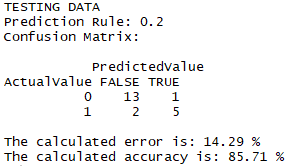
\includegraphics[scale=0.9]{confusion_matrix_final}
	\caption{Confusion Matrix - Validation Data}
\end{figure}

\begin{table}[H]
	\centering
	\begin{tabular}{ |c|c||c| }
 	\multicolumn{2}{c}{\underline{Disease Status}} \\
 	\hline
 	With High Grade Cancer&Without High Grade Cancer&Total\\
 	28.6\%&7.1\%&14.3\%\\
 	\hline
	\end{tabular}
 	\caption{Percent Prediction Error Rates - Validation Data}
\end{table}

Note that the total prediction error rate of 14.3\% is approximately equal to, or very similar to, the 15.8\% error rate based on the model-building data set. Therefore the latter is a reliable indicator of the predictive capability of the fitted logistic regression model and the chosen prediction rule. The accuracy is seen to be 85.7\%.

\subsection{Final Remarks}
The primary purpose of this study was to assess the strength of the association between each of the predictor variables with the response variable, the predictable nature of PSA Level, and the probability of a man having been diagnosed with high grade prostate cancer over low grade. We can now examine the odds ratios of the fitted model (Eqn. 7) to help address these questions. \par
The interpretation for multiple logistic regression is that the estimated odds ratio for the predictor variable \(X_k\) assumes that all other predictor variables are held constant. In view of the fitted model (Eqn. 7) the estimated coefficients are: \(\hat{\beta}_0 = -2.6867\), \(\hat{\beta}_1 = 1.0577\), and \(\hat{\beta}_2 = 1.5502\).
Therefore we can see, for instance, that the odds of a man being diagnosed with high grade prostate cancer increase by about 5.8\% for each additional score of PSA Level, for a given Cancer Volume. This means each unit increase of PSA Level increases the odds of said diagnosis by 5.8\%. Similarly, the odds of a man being diagnosed with high grade prostate cancer increase by  55.0\% for each unit increase in cancer volume. \par 
Thus, these calculated odds ratios suggest that Cancer Volume has a significantly larger association to the outcome (a diagnosis of high grade prostate cancer) than PSA Level. However, PSA Level proved more significant than all other predictors in my analysis of \S4.2, was used to achieve 85.7\% accuracy against validation data in \S5.1, and is both a cost-effective and noninvasive screening procedure for prostate cancer grade classification. \par
Lastly, because this study is observational by nature (all 97 selected men were predetermined to have been diagnosed with prostate cancer), we must be careful about the scope of inferences we draw. Since the data are observational, the result cannot be used as proof that high grade patients test with higher PSA Level; the possibility of confounding variables cannot be excluded. Furthermore, since the individuals were not said be be drawn at random from the population of men about to undergo radical prostectomies, inference to a broader population is not justified.
